\documentclass[fleqn]{article}

\usepackage{mathtools}
\usepackage{nccmath}
\usepackage{graphicx}
\usepackage{float}
\usepackage{booktabs}

\usepackage [english]{babel}
\usepackage [autostyle, english = american]{csquotes}
\MakeOuterQuote{"}

\DeclarePairedDelimiter\Floor\lfloor\rfloor
\DeclarePairedDelimiter\Ceil\lceil\rceil

\title{ODE model of the spread of measles in secondary schools}
\author{David Gurevich}
\date{}

\begin{document}
\maketitle

The following introduces a system of differential equations that is used to model the spread of measles through a secondary school.

\section*{List of Symbols}

	$\beta$ - Probability of disease transmission following an interaction \\
	$\sigma$ - Rate of maturation from exposed class to infected class \\ 
	$\alpha$ - Rate at which symptoms appear in an infected individual \\
	$\gamma$ - Rate at which infected individuals recover following the first appearance of \indent symptoms \\
	$\omega$ - Probability of an individual visiting the bathroom \\
	$q$ - Quantity of virus "shed" per minute \\ 
	$Q$ - Ventilation of air inside washroom (per cubic meter) \\
	$V$ - Volume of each washroom (cubic meters) \\
	$P$ - Pulmonary ventilation rate (cubic meters per minute) \\
	$T$ - Average duration of washroom visit \\
	$\mathcal{F}$ - Symmetrical contact matrix for friends between grades \\
	$\mathcal{C}$ - Symmetrical contact matrix for classmates between grades \\

\newpage

\section*{SVEIR Model}

$S_i$ - Proportion of population $i$ that is susceptible \\
$V_i$ - Proportion of population $i$ that is vaccinated \\
$E_i$ - Proportion of population $i$ that is exposed \\
$I_i$ - Proportion of population $i$ that is infected \\
$H_i$ - Proportion of population $i$ that is at home because of infection \\
$R_i$ - Proportion of population $i$ that has recovered \\
$W$ - Sum of all concentrations of measles virus in the air in washrooms\\ \\
$\tau$ - Day state: 1 if students are at home, 2 if students are in the halls, 3 if \indent students are in class
\begin{equation}
\dfrac{dS_i}{dt} = 
\begin{dcases}
	0 & \text{if $\tau = 1$} \\
	- \Big[\Big(\sum_{j=1}^4 \dfrac{2}{20} \beta \mathcal{F}_{i,j} I_j \Big) + \dfrac{1}{6} \omega \beta W P \Big](\dfrac{S_i}{N_i}) & \text{if $\tau = 2$} \\
	- \Big[\Big(\sum_{j=1}^4 \dfrac{2}{20} \beta \mathcal{C}_{i,j} I_j \Big) + \dfrac{1}{6} \omega \beta W P \Big](\dfrac{S_i}{N_i}) & \text{if $\tau = 3$} 	
\end{dcases}
\end{equation}

\begin{equation}
\dfrac{dV_i}{dt} = 0
\end{equation}

\begin{equation}
\dfrac{dE_i}{dt} = 
\begin{dcases}
	0 & \text{if $\tau = 1$} \\
	\Big[\Big(\sum_{j=1}^4 \dfrac{2}{20} \beta \mathcal{F}_{i,j} I_j \Big) + \dfrac{1}{6} \omega \beta W P \Big](\dfrac{S_i}{N_i}) - \sigma E_i & \text{if $\tau = 2$} \\
	\Big[\Big(\sum_{j=1}^4 \dfrac{2}{20} \beta \mathcal{C}_{i,j} I_j \Big) + \dfrac{1}{6} \omega \beta W P \Big](\dfrac{S_i}{N_i}) - \sigma E_i & \text{if $\tau = 3$} 	
\end{dcases}
\end{equation}

\begin{equation}
\dfrac{dI_i}{dt} = \sigma E_i - \alpha I_i
\end{equation}

\begin{equation}
\dfrac{dH_i}{dt} = \alpha I_i - \gamma H_i
\end{equation}

\begin{equation}
\dfrac{dR_i}{dt} = \gamma H_i
\end{equation}

\begin{equation}
\dfrac{dW}{dt} = 
\begin{dcases}
\dfrac{-Q}{V} & \text{if $\tau = 1$} \\
\dfrac{-Q}{V} + \dfrac{1}{6} \omega q T \sum_{j=1}^4 I_j & \text{if $\tau = 2, 3$}
\end{dcases}
\end{equation}

\newpage

\begin{figure}[t!]
	\vspace*{-1.5in}
	\hspace{-2.7in}
	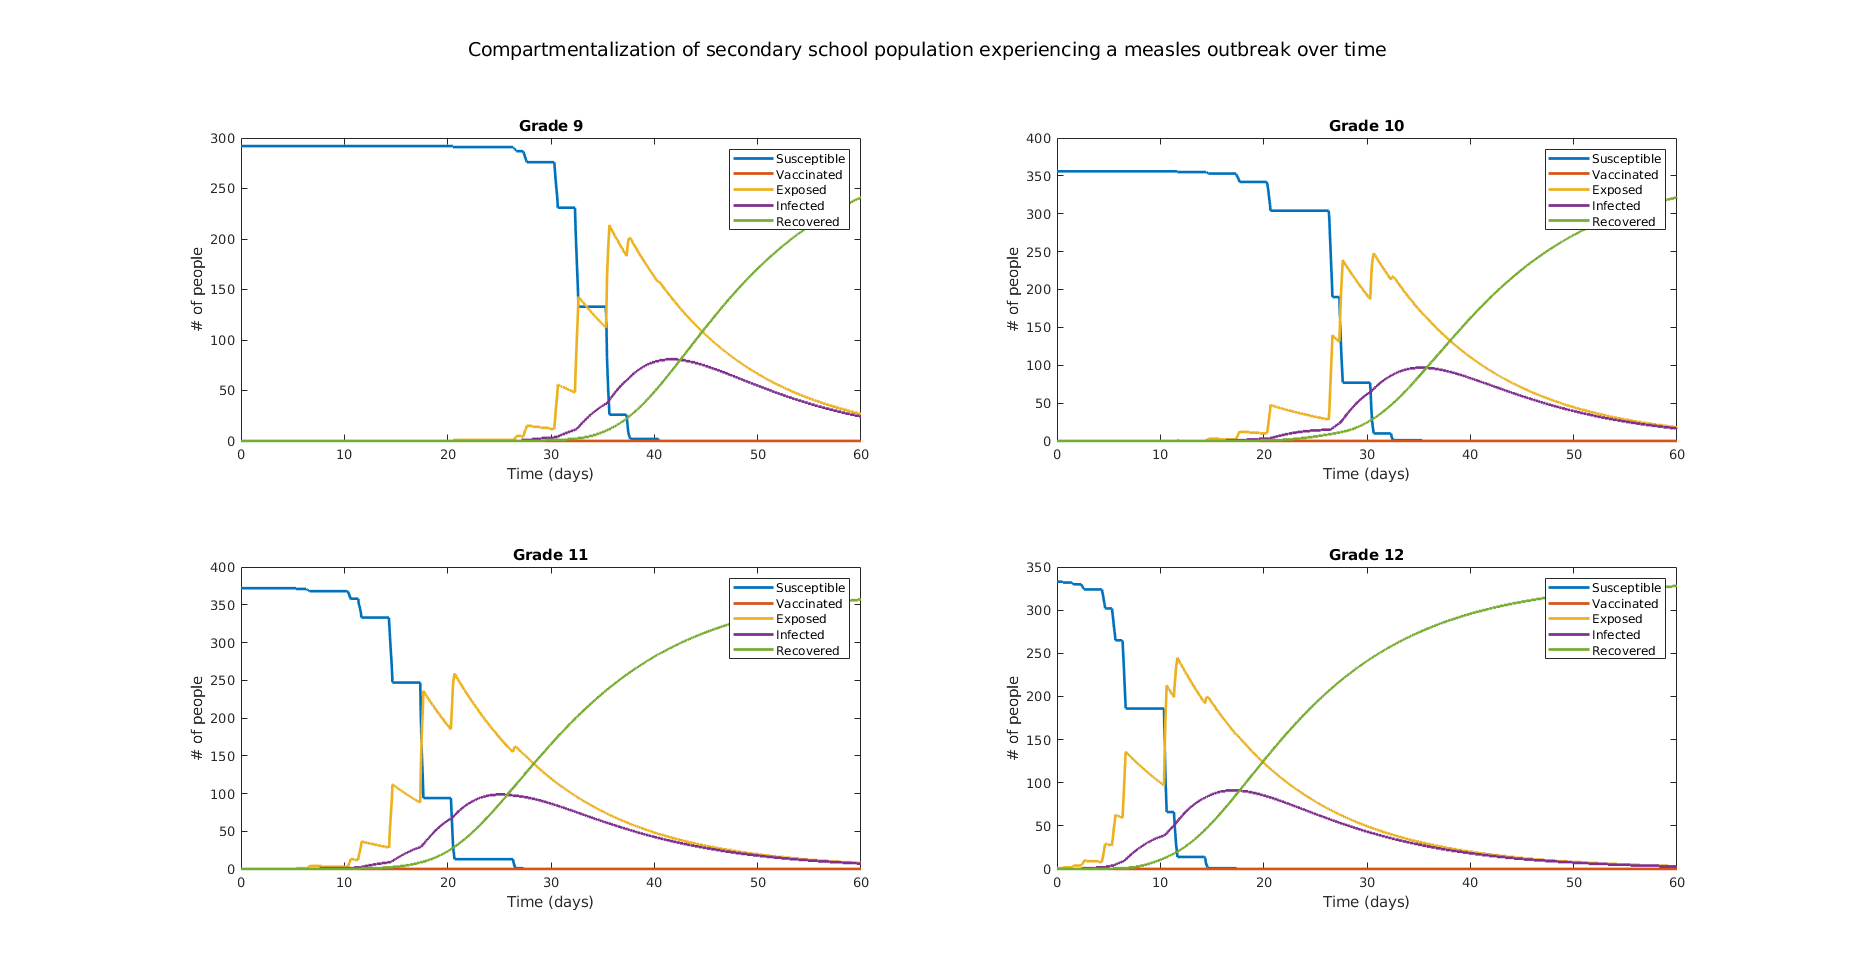
\includegraphics[scale=0.52]{fig.png}
\end{figure}
\begin{center}
Figure 1: Plot of ODE solution to model
\begin{table}[h]
\begin{tabular}{@{}cccc@{}}
$\beta$ = 0.91                                                                                                                                                     & $\dfrac{1}{\gamma}$ = 4 & $Q$ = 5                                                          & $T$ = 2.2                                                        \\
$\dfrac{1}{\sigma}$ = 11                                                                                                                                            & $\omega$ = 0.00047     & $V$ = 32                                                         &                                                                  \\[0.4cm]
$\dfrac{1}{\alpha}$ = 4                                                                                                                                             & $q$ = 144              & $P$ = 0.00556                                                    &                                                                  \\
\multicolumn{1}{l}{}                                                                                                                                               & \multicolumn{1}{l}{}   & \multicolumn{1}{l}{}                                             & \multicolumn{1}{l}{}                                             \\
\multicolumn{1}{l}{$ \mathcal{F} = \begin{bmatrix} 0.97 & 0.03 & 0 & 0 \\ 0.03 & 0.97 & 0.03 & 0 \\ 0 & 0.03 & 0.097 & 0.03 \\ 0 & 0 & 0.03 & 0.97 \end{bmatrix}$} & \multicolumn{1}{l}{}   & \multicolumn{2}{l}{$ \mathcal{C} = \begin{bmatrix} 1 & 0 & 0 & 0 \\ 0 & 1 & 0 & 0 \\ 0 & 0 & 1 & 0 \\ 0 & 0 & 0 & 1 \end{bmatrix}$}
\end{tabular}
\end{table}

\end{center}


\end{document}